\documentclass[12pt,a4paper]{article}
\usepackage[UTF8]{ctex}
\usepackage{geometry}
\usepackage{graphicx}
\usepackage{booktabs}
\usepackage{longtable}
\usepackage{array}
\usepackage{multirow}
\usepackage{amsmath}
\usepackage{hyperref}
\usepackage{xcolor}
\usepackage{tikz}
\usepackage{enumitem}
\usepackage{fancyhdr}
\usepackage{titlesec}
\usepackage{tabularx}
\usepackage{caption}
\usepackage{algorithm}
\usepackage{algpseudocode}

\geometry{left=2.5cm, right=2.5cm, top=2.8cm, bottom=2.5cm}

\pagestyle{fancy}
\fancyhf{}
\fancyhead[L]{\small 软件项目开发与实践}
\fancyhead[R]{\small 设计与实现文档}
\fancyfoot[C]{\thepage}
\renewcommand{\headrulewidth}{0.4pt}

\titleformat{\section}{\Large\bfseries\color{blue!70!black}}{第\,\thesection\,章}{0.8em}{}
\titleformat{\subsection}{\large\bfseries}{}{0em}{}
\titleformat{\subsubsection}{\normalsize\bfseries}{}{0em}{}

\begin{document}

\begin{titlepage}
\centering
\vspace*{3cm}
{\Huge\bfseries\color{blue!70!black} 星露谷战斗模块}\\[0.8cm]
{\LARGE\color{blue!50!black} 俯视角像素风动作角色扮演游戏}\\[0.5cm]
{\large\color{gray} --- 以《星露谷物语》矿洞战斗为灵感 ---}\\[3cm]
{\Large 项目设计与实现文档}\\[2cm]
\renewcommand{\arraystretch}{1.8}
\begin{tabular}{rl}
\textbf{课程名称：} & 软件项目开发与实践 \\
\textbf{项目名称：} & 星露谷战斗模块 \\
\textbf{姓\quad 名：} & 谢宇鹏 \\
\textbf{学\quad 号：} & 5120243390 \\
\textbf{开发模式：} & B模式（AI智能协作开发） \\
\textbf{技术栈：} & Python + Pygame \\
\textbf{文档版本：} & V1.0 \\
\end{tabular}
\vfill
{\small 本文档阐述系统架构设计、面向对象类结构、核心算法分析和测试方案。}
\end{titlepage}

\tableofcontents
\newpage

% ============================================================
% 第1章 系统架构设计
% ============================================================
\section{系统架构设计}

\subsection{架构风格选择}

经过对多种架构风格的对比分析，本项目采用\textbf{分层架构}（Layered Architecture），结合面向对象设计原则。

\begin{table}[htbp]
\centering
\begin{tabularx}{\textwidth}{lXX}
\toprule
\textbf{架构风格} & \textbf{优点} & \textbf{缺点} \\
\midrule
分层架构 & 职责清晰，上下层解耦，易于测试和维护 & 层间通信有一定开销 \\
MVC & 模型视图分离 & 对实时游戏循环不太自然 \\
ECS & 高性能，数据驱动 & 实现复杂度高，不适合小项目 \\
事件驱动 & 松耦合，扩展性好 & 调试困难，流程不直观 \\
\bottomrule
\end{tabularx}
\end{table}

\textbf{选择理由}：分层架构最适合本项目的规模和复杂度——层级清晰、职责明确、团队协作方便。

\subsection{系统组件图}

\begin{figure}[htbp]
\centering
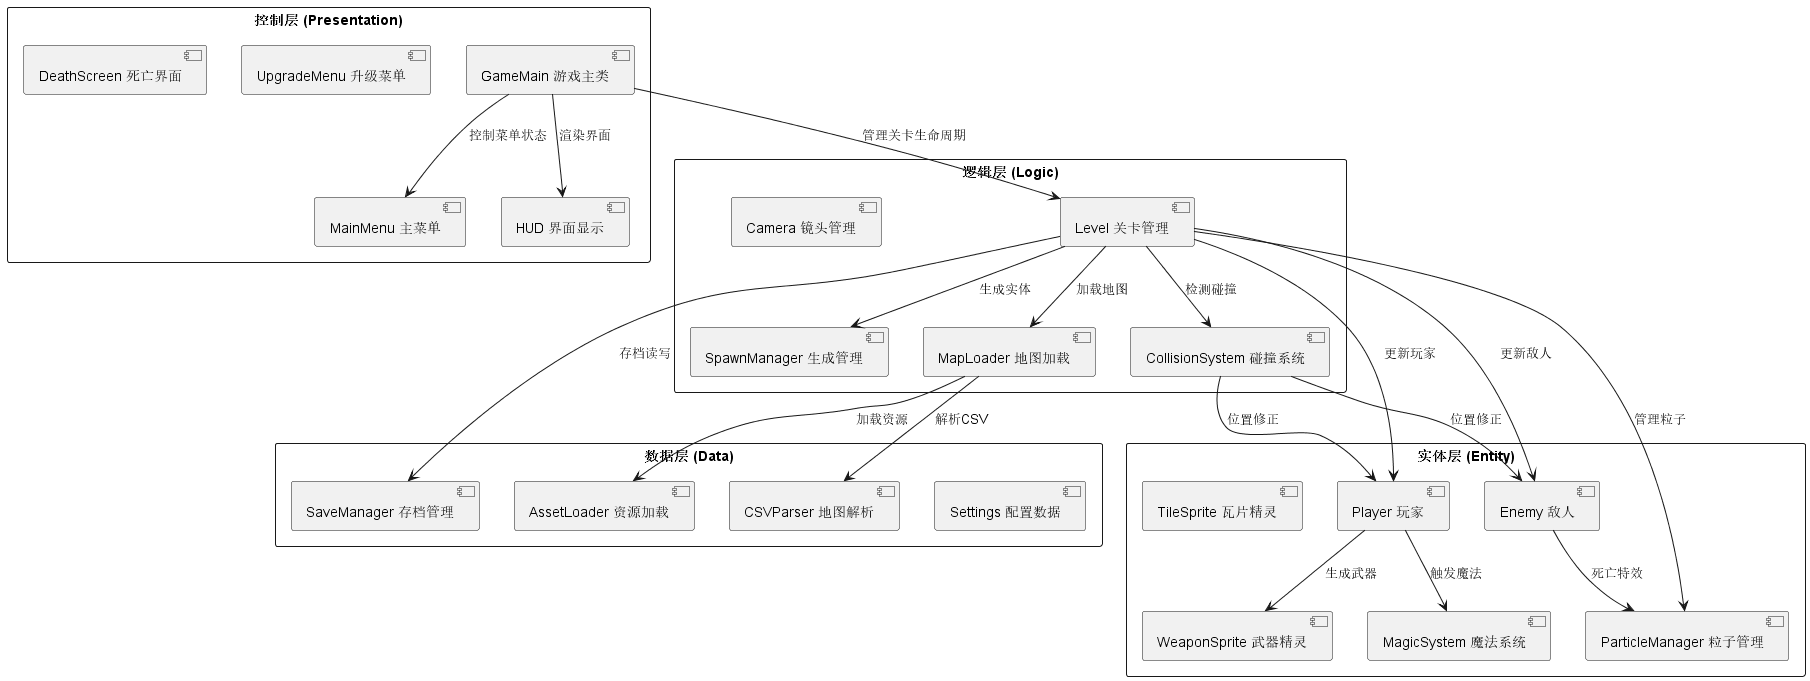
\includegraphics[width=0.95\textwidth]{fig/组件图.png}
\caption{系统组件图（PlantUML生成）}
\label{fig:component}
\end{figure}

系统分为四层：
\begin{itemize}[leftmargin=2em]
    \item \textbf{控制层}：GameMain游戏主类、MainMenu主菜单、HUD界面显示、UpgradeMenu升级菜单、DeathScreen死亡界面
    \item \textbf{逻辑层}：Level关卡管理、MapLoader地图加载、Camera镜头管理、CollisionSystem碰撞系统、SpawnManager生成管理
    \item \textbf{实体层}：Player玩家、Enemy敌人、WeaponSprite武器精灵、MagicSystem魔法系统、ParticleManager粒子管理、TileSprite瓦片精灵
    \item \textbf{数据层}：Settings配置数据、SaveManager存档管理、CSVParser地图解析、AssetLoader资源加载
\end{itemize}

\subsection{分层职责说明}

\begin{table}[htbp]
\centering
\begin{tabularx}{\textwidth}{lXX}
\toprule
\textbf{层级} & \textbf{职责} & \textbf{包含模块} \\
\midrule
控制层 & 游戏主循环、状态机、输入事件、菜单渲染 & GameMain, MainMenu, HUD, UpgradeMenu, DeathScreen \\
逻辑层 & 关卡管理、地图加载、碰撞检测、场景切换、实体生成 & Level, MapLoader, Camera, CollisionSystem, SpawnManager \\
实体层 & 玩家、敌人、武器、魔法、粒子、瓦片精灵 & Player, Enemy, WeaponSprite, MagicSystem, ParticleManager, TileSprite \\
数据层 & 配置数据、存档读写、地图解析、资源加载 & Settings, SaveManager, CSVParser, AssetLoader \\
\bottomrule
\end{tabularx}
\end{table}

\textbf{设计原则}：
\begin{enumerate}[leftmargin=2em]
    \item 上层依赖下层，下层不依赖上层（依赖倒置）
    \item 同层之间通过回调函数通信，避免直接引用
    \item 每个模块职责单一，符合SRP原则
\end{enumerate}


% ============================================================
% 第2章 面向对象设计
% ============================================================
\section{面向对象设计}

\subsection{设计原则应用}

\begin{table}[htbp]
\centering
\begin{tabularx}{\textwidth}{lXX}
\toprule
\textbf{原则} & \textbf{在本项目中的体现} & \textbf{设计目的} \\
\midrule
封装 & 每个类管理自己的状态，外部通过方法交互 & 隐藏实现细节，降低耦合 \\
继承 & 玩家和敌人继承实体基类，复用移动和碰撞代码 & 代码复用，减少重复 \\
多态 & 同一移动方法在不同子类中表现不同（键盘驱动 vs AI驱动） & 统一接口，灵活扩展 \\
组合 & 关卡类组合管理玩家、敌人、武器等对象 & 灵活装配，职责分离 \\
单一职责 & 每个类只负责一个功能域 & 降低复杂度，便于维护 \\
\bottomrule
\end{tabularx}
\end{table}

\subsection{类图设计}

\begin{figure}[htbp]
\centering
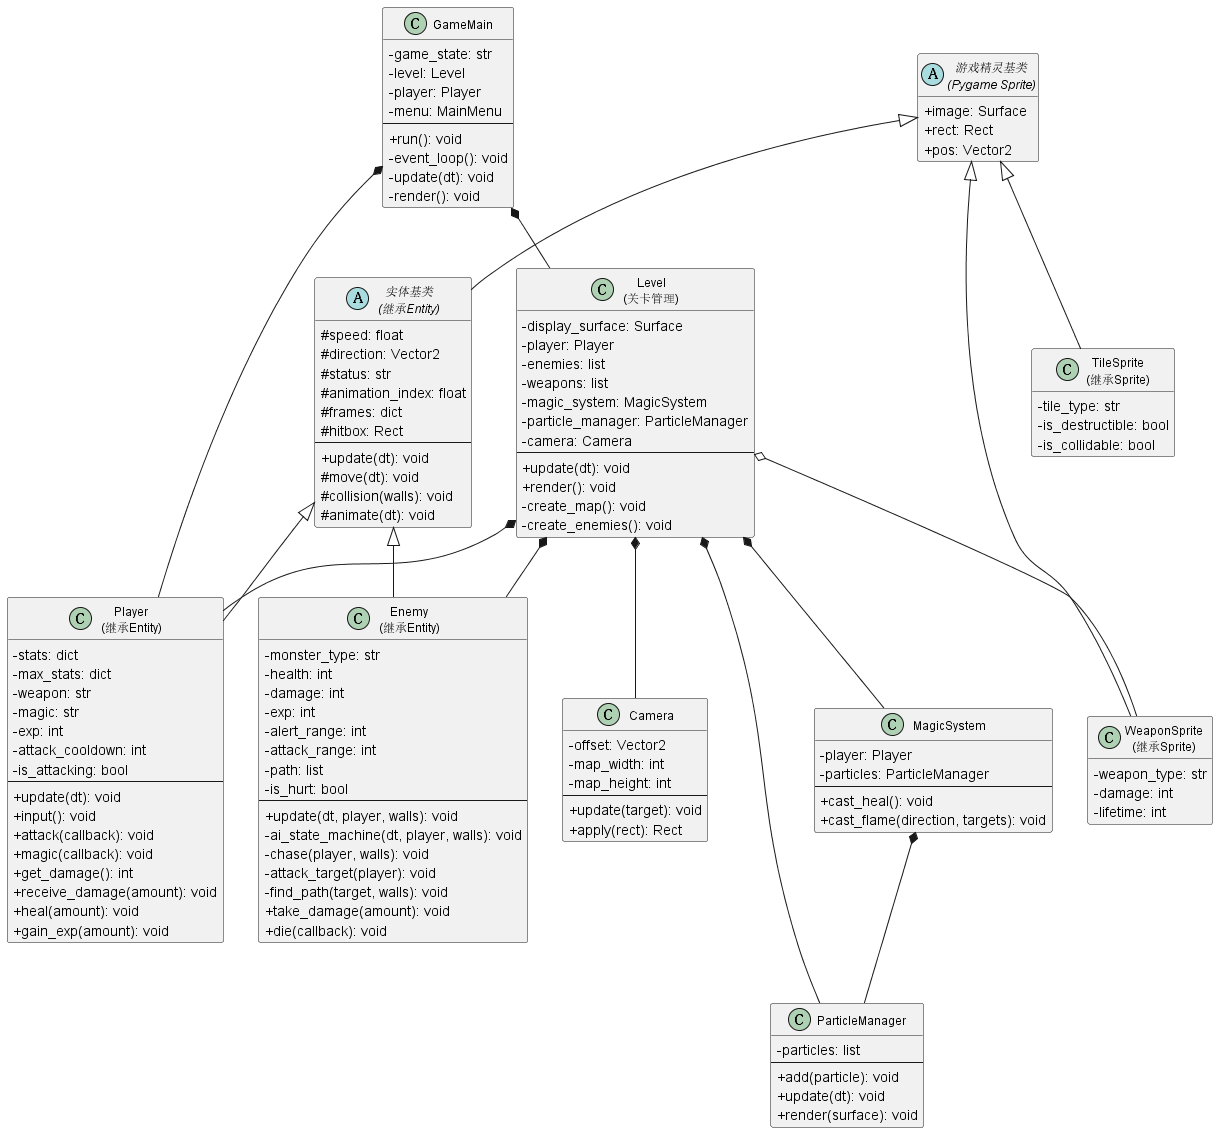
\includegraphics[width=0.95\textwidth]{fig/类图.png}
\caption{类图——继承与组合关系（PlantUML生成）}
\label{fig:class}
\end{figure}

\subsection{类职责详述}

\subsubsection{游戏精灵基类（Sprite）}

Pygame的Sprite基类的封装，提供统一的图像加载和矩形更新接口。所有可视对象继承此类。

\subsubsection{实体基类（Entity）}

封装公共行为：
\begin{itemize}[leftmargin=2em]
    \item \textbf{统一移动}：速度 $\times$ 方向向量 $\times$ 帧时间
    \item \textbf{分轴碰撞}：先水平后垂直，避免对角线穿墙
    \item \textbf{Hitbox}：缩小碰撞框，比精灵图像小一圈，提升碰撞精度
    \item \textbf{动画帧管理}：浮点索引累加，支持不同帧数的动画混合
\end{itemize}

\subsubsection{玩家类（Player）}

输入驱动型角色：
\begin{itemize}[leftmargin=2em]
    \item 键盘输入 $\rightarrow$ 设置方向 $\rightarrow$ 切换动画状态
    \item 攻击/魔法触发通过回调通知关卡层
    \item 冷却管理通过时间戳差值判断
    \item 能量每帧自动恢复
\end{itemize}

\subsubsection{敌人类（Enemy）}

AI驱动型角色：
\begin{itemize}[leftmargin=2em]
    \item 三态状态机（待机/追踪/攻击），根据玩家距离切换
    \item 追踪时调用寻路算法，路径缓存 + 定时重算
    \item 死亡时通知关卡层播放特效、增加经验值
\end{itemize}

\subsubsection{关卡管理类（Level）}

核心协调者：
\begin{itemize}[leftmargin=2em]
    \item 地图解析 $\rightarrow$ 实体创建 $\rightarrow$ 碰撞调度 $\rightarrow$ 传送管理 $\rightarrow$ 存档接口
    \item 管理所有实体的更新和渲染顺序
    \item 处理玩家攻击和魔法的回调
\end{itemize}


% ============================================================
% 第3章 核心算法分析
% ============================================================
\section{核心算法分析}

\subsection{智能寻路算法}

\subsubsection{问题建模}

敌人需要在网格地图上找到一条从自身位置到玩家位置的路径，且该路径必须绕过障碍物（树木、石墙等不可通行格子）。

设地图为 $M \times N$ 的网格，每个格子状态为「可通行」或「不可通行」。起点为敌人位置 $S$，终点为玩家位置 $G$。目标：找到从 $S$ 到 $G$ 的最短路径（步数最少）。

\subsubsection{候选算法分析}

\paragraph{候选一：广度优先搜索（BFS）}

从起点开始逐层扩展，先访问所有距离为1的节点，再访问距离为2的节点，直到找到终点。

\begin{itemize}[leftmargin=2em]
    \item \textbf{优点}：一定能找到最短路径，实现简单，无需设计启发函数
    \item \textbf{缺点}：无方向性，盲目扩展所有方向（上/下/左/右/对角线），搜索范围大
    \item \textbf{时间复杂度}：$O(V + E)$，$V$为节点数，$E$为边数
    \item \textbf{空间复杂度}：$O(V)$
    \item \textbf{适用性}：适合无权图的最短路径，但效率偏低
\end{itemize}

\paragraph{候选二：Dijkstra算法}

从起点开始，每次选择当前累计代价最小的节点扩展，逐步到达终点。

\begin{itemize}[leftmargin=2em]
    \item \textbf{优点}：保证最短路径，支持加权图（不同地形移动代价不同）
    \item \textbf{缺点}：无启发式引导，搜索范围仍较大，向所有方向均匀扩展
    \item \textbf{时间复杂度}：$O((V + E) \log V)$，使用优先队列
    \item \textbf{适用性}：本项目网格权重相同，Dijkstra的加权能力用不上
\end{itemize}

\paragraph{候选三：A*算法（最终选择）}

综合Dijkstra和贪心搜索，使用评估函数引导搜索方向：
\[f(n) = g(n) + h(n)\]
其中 $g(n)$ 为起点到当前节点的实际代价，$h(n)$ 为当前节点到终点的启发式估计。

\begin{itemize}[leftmargin=2em]
    \item \textbf{启发函数}：曼哈顿距离 $h(n) = |x_1 - x_2| + |y_1 - y_2|$
    \item \textbf{优点}：保证最短路径（启发函数满足一致性条件时），启发式剪枝大幅减少搜索范围
    \item \textbf{缺点}：需要设计合适的启发函数，最坏情况退化为Dijkstra
    \item \textbf{时间复杂度}：最坏 $O(E)$，实际远小于此
    \item \textbf{空间复杂度}：$O(V)$
    \item \textbf{适用性}：本项目的最佳选择——网格地图、静态障碍物、需最短路径
\end{itemize}

\paragraph{候选四：贪心最佳优先搜索}

每次只考虑启发函数 $h(n)$，选择离终点最近的节点扩展。

\begin{itemize}[leftmargin=2em]
    \item \textbf{优点}：搜索速度极快，直奔目标方向
    \item \textbf{缺点}：不保证最短路径，可能走入死胡同后需要回溯
    \item \textbf{时间复杂度}：$O(E)$
    \item \textbf{适用性}：速度最快但路径质量无保证，不适合本项目
\end{itemize}

\subsubsection{算法选型对比}

\begin{table}[htbp]
\centering
\begin{tabularx}{\textwidth}{lXXXXX}
\toprule
\textbf{算法} & \textbf{最短路径} & \textbf{搜索效率} & \textbf{实现难度} & \textbf{动态地图} & \textbf{本项目适用性} \\
\midrule
BFS & 保证 & 低 & 简单 & 支持 & 不推荐 \\
Dijkstra & 保证 & 中 & 中等 & 支持 & 可用 \\
\textbf{A*} & \textbf{保证} & \textbf{高} & 中等 & \textbf{支持} & \textbf{最终选择} \\
贪心搜索 & 不保证 & 极高 & 简单 & 支持 & 不推荐 \\
\bottomrule
\end{tabularx}
\end{table}

\subsubsection{A*算法伪代码}

\begin{algorithm}[htbp]
\caption{A*寻路算法}
\begin{algorithmic}[1]
\Require 起点 $S$, 终点 $G$, 地图 $M$
\Ensure 从 $S$ 到 $G$ 的最短路径
\State open\_list $\leftarrow$ 优先队列，按 $f(n)$ 排序
\State closed\_set $\leftarrow$ 空集合
\State $g(S) \leftarrow 0$, $f(S) \leftarrow h(S)$
\State 将 $S$ 加入 open\_list
\While{open\_list 非空}
    \State $current \leftarrow$ open\_list 中 $f$ 值最小的节点
    \If{$current = G$}
        \State \Return 回溯重建路径
    \EndIf
    \State 将 $current$ 从 open\_list 移入 closed\_set
    \For{每个相邻节点 $neighbor$}
        \If{$neighbor$ 不可通行 或 $neighbor \in closed\_set$}
            \State \textbf{continue}
        \EndIf
        \State $tentative\_g \leftarrow g(current) + 1$
        \If{$neighbor \notin open\_list$ 或 $tentative\_g < g(neighbor)$}
            \State $g(neighbor) \leftarrow tentative\_g$
            \State $f(neighbor) \leftarrow g(neighbor) + h(neighbor)$
            \State 记录 $neighbor$ 的父节点为 $current$
            \State 将 $neighbor$ 加入 open\_list
        \EndIf
    \EndFor
\EndWhile
\State \Return 空路径（无法到达）
\end{algorithmic}
\end{algorithm}

\subsubsection{性能优化策略}

\begin{enumerate}[leftmargin=2em]
    \item \textbf{路径缓存}：计算好的路径保存起来，每隔500ms或玩家移动到新网格时才重新计算，避免每帧计算
    \item \textbf{搜索范围限制}：当搜索距离超过一定阈值时停止，防止在大地图上搜索耗时过长
    \item \textbf{曼哈顿距离}：使用曼哈顿距离而非欧几里得距离，减少浮点运算开销
\end{enumerate}

\subsection{分轴AABB碰撞检测}

\subsubsection{问题分析}

在2D游戏中，角色移动通常是同时更新$x$和$y$坐标。如果在一次碰撞检测中同时处理两个轴，角色可能在对角线方向同时穿过两个相邻障碍物的夹角。

\subsubsection{解决方案}

将二维碰撞分解为两个一维碰撞，分两步处理：

\begin{enumerate}[leftmargin=2em]
    \item \textbf{水平方向}：更新$x$坐标后，检测水平方向碰撞，若碰撞则将$x$回退到障碍物边界
    \item \textbf{垂直方向}：更新$y$坐标后，检测垂直方向碰撞，若碰撞则将$y$回退到障碍物边界
\end{enumerate}

\begin{algorithm}[htbp]
\caption{分轴碰撞检测}
\begin{algorithmic}[1]
\Require 角色位置 $(x, y)$, 速度 $(v_x, v_y)$, 墙壁集合 $W$, 帧时间 $\Delta t$
\Ensure 修正后的位置 $(x', y')$
\State $x \leftarrow x + v_x \cdot \Delta t$ \Comment{更新水平位置}
\State $hitbox.x \leftarrow x$ \Comment{更新碰撞框}
\For{每个墙壁 $wall \in W$}
    \If{$hitbox$ 与 $wall.rect$ 重叠}
        \If{$v_x > 0$} \Comment{向右移动}
            \State $hitbox.right \leftarrow wall.rect.left$
        \ElsIf{$v_x < 0$} \Comment{向左移动}
            \State $hitbox.left \leftarrow wall.rect.right$
        \EndIf
    \EndIf
\EndFor
\State $x \leftarrow hitbox.x - hitbox\_offset.x$ \Comment{同步位置}
\State $y \leftarrow y + v_y \cdot \Delta t$ \Comment{更新垂直位置}
\State $hitbox.y \leftarrow y$ \Comment{更新碰撞框}
\For{每个墙壁 $wall \in W$}
    \If{$hitbox$ 与 $wall.rect$ 重叠}
        \If{$v_y > 0$} \Comment{向下移动}
            \State $hitbox.bottom \leftarrow wall.rect.top$
        \ElsIf{$v_y < 0$} \Comment{向上移动}
            \State $hitbox.top \leftarrow wall.rect.bottom$
        \EndIf
    \EndIf
\EndFor
\State $y \leftarrow hitbox.y - hitbox\_offset.y$ \Comment{同步位置}
\State \Return $(x, y)$
\end{algorithmic}
\end{algorithm}

\textbf{为什么分轴}：若同时处理两个轴，角色在$(v_x, v_y) = (1, 1)$方向移动时，可能同时穿过水平和垂直方向的两个障碍物夹角。分轴处理从根本上避免了对角线穿墙问题。

\subsection{Y轴排序渲染}

\subsubsection{问题分析}

在俯视角游戏中，为了实现正确的遮挡关系（画面下方的角色挡住上方的角色），需要按照Y坐标排序后绘制。

\subsubsection{解决方案}

\begin{enumerate}[leftmargin=2em]
    \item 计算相机偏移量：以玩家位置为中心
    \item 绘制地面贴图（最底层）
    \item 将所有可见精灵（玩家、敌人、草地、瓦片等）收集到一个列表
    \item 按Y坐标排序（Y值大的排后面）
    \item 按排序顺序依次绘制，Y值大的后绘制（覆盖Y值小的）
\end{enumerate}

\subsection{有限状态机（FSM）}

\subsubsection{敌人AI状态机}

\begin{figure}[htbp]
\centering
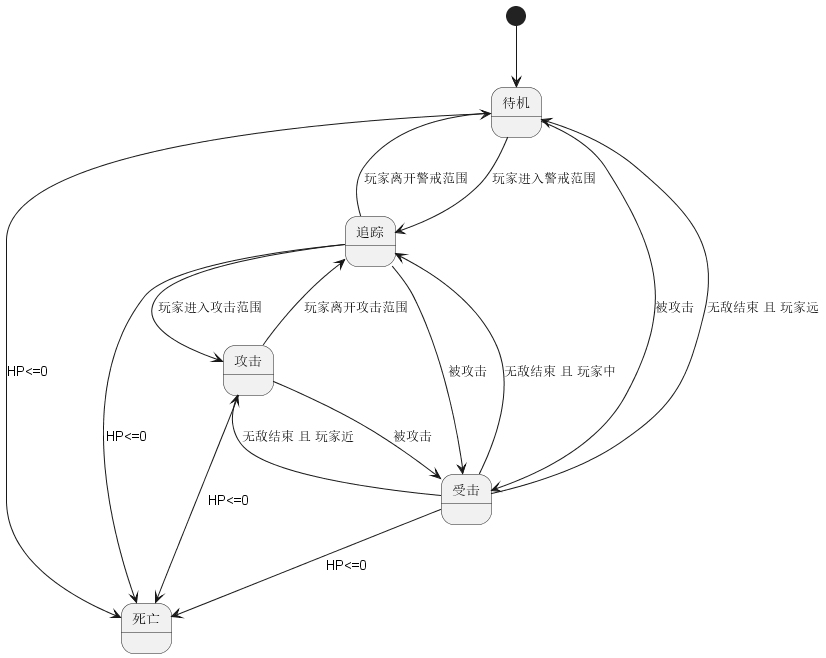
\includegraphics[width=0.85\textwidth]{fig/敌人AI状态机.png}
\caption{敌人AI有限状态机（PlantUML生成）}
\label{fig:enemy_fsm}
\end{figure}

敌人AI包含五个状态：待机、追踪、攻击、受击、死亡。状态转换由玩家距离和自身HP决定。

\subsubsection{游戏主流程状态机}

\begin{figure}[htbp]
\centering
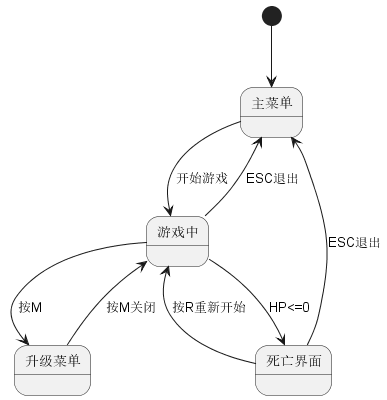
\includegraphics[width=0.7\textwidth]{fig/游戏流程状态机.png}
\caption{游戏主流程状态机（PlantUML生成）}
\label{fig:game_fsm}
\end{figure}

游戏主流程包含四个状态：主菜单、游戏中、死亡界面、升级菜单。


% ============================================================
% 第4章 关键交互时序
% ============================================================
\section{关键交互时序}

\subsection{近战攻击时序图}

\begin{figure}[htbp]
\centering
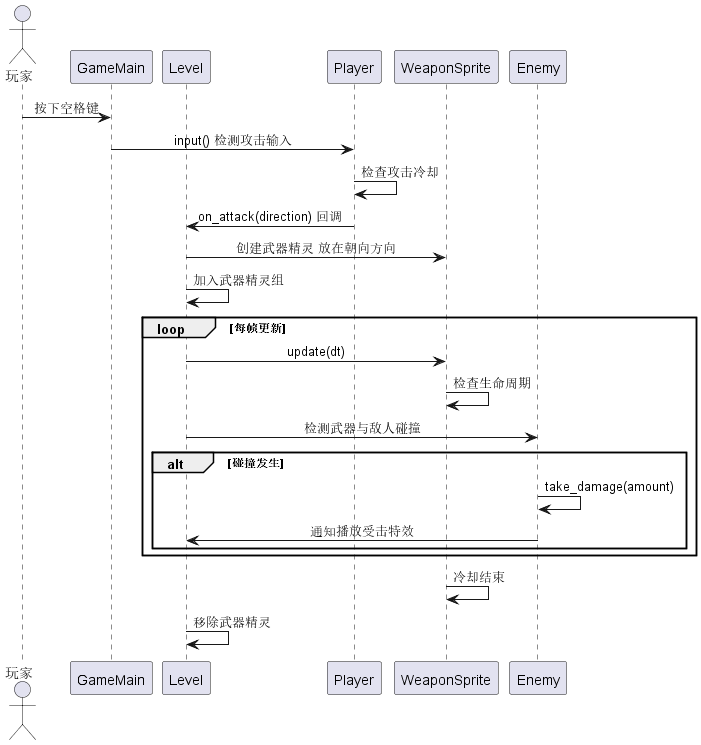
\includegraphics[width=0.9\textwidth]{fig/攻击时序图.png}
\caption{近战攻击时序图（PlantUML生成）}
\label{fig:attack_seq}
\end{figure}

攻击流程：玩家按空格 $\rightarrow$ Player检测冷却 $\rightarrow$ 回调Level创建武器精灵 $\rightarrow$ 每帧检测碰撞 $\rightarrow$ 碰撞发生则Enemy扣血 $\rightarrow$ 冷却结束移除武器。

\subsection{场景切换时序图}

\begin{figure}[htbp]
\centering
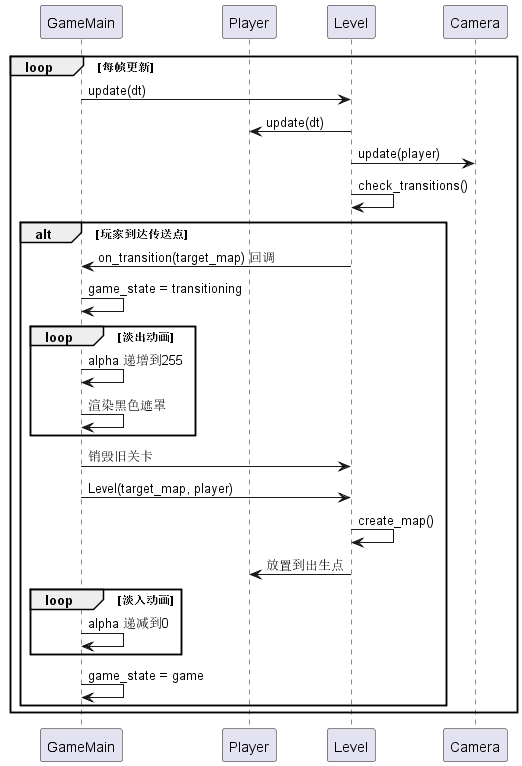
\includegraphics[width=0.9\textwidth]{fig/场景切换时序图.png}
\caption{场景切换时序图（PlantUML生成）}
\label{fig:scene_seq}
\end{figure}

切换流程：检测传送点 $\rightarrow$ 回调GameMain $\rightarrow$ 淡出动画 $\rightarrow$ 销毁旧关卡 $\rightarrow$ 创建新Level $\rightarrow$ 加载新地图 $\rightarrow$ 淡入动画。

\subsection{怪物AI行为时序图}

\begin{figure}[htbp]
\centering
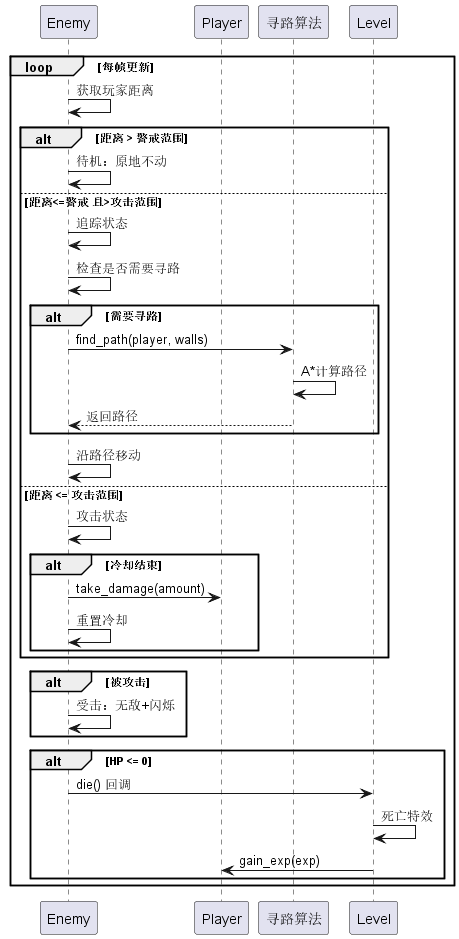
\includegraphics[width=0.9\textwidth]{fig/怪物AI时序图.png}
\caption{怪物AI行为时序图（PlantUML生成）}
\label{fig:enemy_seq}
\end{figure}

AI流程：每帧获取玩家距离 $\rightarrow$ 判断状态 $\rightarrow$ 待机/追踪/攻击 $\rightarrow$ 追踪时调用寻路算法 $\rightarrow$ 被攻击进入受击状态 $\rightarrow$ HP$\leq$0则死亡。


% ============================================================
% 第5章 数据结构设计
% ============================================================
\section{数据结构设计}

\subsection{配置数据结构}

武器、怪物、魔法数据采用字典嵌套结构，实现数据驱动设计。新增内容无需修改核心代码，只需添加配置条目。

\begin{table}[htbp]
\centering
\begin{tabularx}{\textwidth}{lXX}
\toprule
\textbf{数据类型} & \textbf{结构} & \textbf{字段} \\
\midrule
武器 & dict[str, dict] & damage, cooldown, graphic, sound \\
怪物 & dict[str, dict] & health, damage, speed, exp, attack\_type, size, hitbox \\
魔法 & dict[str, dict] & strength, cost, graphic, sound \\
\bottomrule
\end{tabularx}
\end{table}

\subsection{地图数据结构}

每张地图由四个CSV文件组成：

\begin{table}[htbp]
\centering
\begin{tabularx}{\textwidth}{lXX}
\toprule
\textbf{文件} & \textbf{数据类型} & \textbf{特殊值} \\
\midrule
ground.csv & int[][] & 各值对应地面瓦片编号 \\
grass.csv & int[][] & 1=可破坏草地 \\
collision.csv & int[][] & 0=可通行, 1=不可通行, 特殊值=出生点/敌人/传送点 \\
entities.csv & int[][] & 特殊值标识敌人类型和传送目标 \\
\bottomrule
\end{tabularx}
\end{table}

\subsection{存档数据结构}

JSON格式，序列化玩家状态和世界状态：

\begin{table}[htbp]
\centering
\begin{tabularx}{\textwidth}{lXX}
\toprule
\textbf{字段} & \textbf{类型} & \textbf{说明} \\
\midrule
player.position & [float, float] & 玩家坐标 \\
player.health & int & 当前生命值 \\
player.energy & int & 当前能量值 \\
player.exp & int & 当前经验值 \\
player.stats & dict & 五项属性值 \\
player.weapon & str & 当前装备武器 \\
current\_map & str & 当前地图ID \\
defeated\_enemies & list[[int,int]] & 已击败敌人坐标 \\
destroyed\_grass & list[[int,int]] & 已破坏草地坐标 \\
\bottomrule
\end{tabularx}
\end{table}


% ============================================================
% 第6章 场景交互设计
% ============================================================
\section{场景交互设计}

\subsection{场景状态转换图}

\begin{figure}[htbp]
\centering
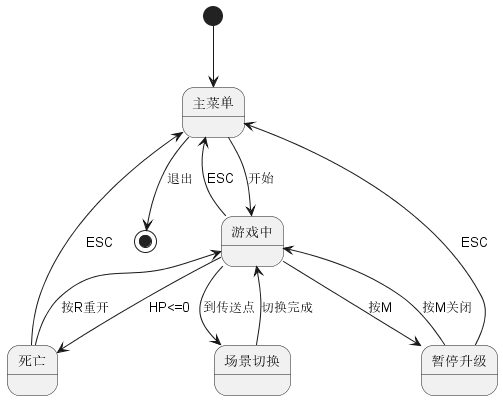
\includegraphics[width=0.9\textwidth]{fig/场景状态转换图.png}
\caption{场景状态转换图（PlantUML生成）}
\label{fig:scene_fsm}
\end{figure}

\subsection{各场景详细设计}

\subsubsection{主菜单场景}

\begin{itemize}[leftmargin=2em]
    \item \textbf{背景渲染}：深蓝色渐变（RGB: 20, 20, 40），浮动蓝色粒子
    \item \textbf{标题动画}：金色文字，正弦函数浮动 $y = A \sin(\omega t + \phi)$
    \item \textbf{菜单选择}：上下键移动高亮，选中项脉冲闪烁（每100ms切换）
    \item \textbf{音频}：背景音乐循环播放
\end{itemize}

\subsubsection{游戏关卡场景}

\begin{itemize}[leftmargin=2em]
    \item \textbf{地图渲染}：地面 $\rightarrow$ 草地 $\rightarrow$ 装饰 $\rightarrow$ 实体，四层叠加
    \item \textbf{视窗系统}：以玩家为中心截取地图局部，计算相机偏移量并限制在地图范围内
    \item \textbf{实体更新}：玩家 $\rightarrow$ 敌人 $\rightarrow$ 武器 $\rightarrow$ 魔法 $\rightarrow$ 粒子，按顺序更新
    \item \textbf{碰撞调度}：实体与墙壁碰撞、武器与敌人碰撞、玩家与传送点碰撞
    \item \textbf{HUD}：屏幕顶部固定绘制血条/能量条/武器图标/经验值
\end{itemize}

\subsubsection{死亡界面}

\begin{itemize}[leftmargin=2em]
    \item \textbf{背景}：暗红色（RGB: 40, 0, 0），红色浮动粒子
    \item \textbf{标题}：红色大字「You Died」
    \item \textbf{统计}：显示本局获得经验值
    \item \textbf{选项}：按R重新开始 / 按ESC退出
\end{itemize}


% ============================================================
% 第7章 测试方案
% ============================================================
\section{测试方案}

\subsection{功能测试}

\begin{longtable}{p{0.5cm}p{2.5cm}p{5cm}p{2cm}p{2cm}}
\toprule
\textbf{编号} & \textbf{测试项} & \textbf{测试内容} & \textbf{预期结果} & \textbf{优先级} \\
\midrule
\endhead
FT-01 & 主菜单显示 & 启动游戏，检查菜单是否正常显示 & 3秒内显示菜单，音乐播放 & P0 \\
FT-02 & 菜单导航 & 上下键选择，回车确认 & 选择正确响应 & P0 \\
FT-03 & 玩家移动 & 四方向移动测试 & 流畅移动，动画正确 & P0 \\
FT-04 & 碰撞检测 & 靠近墙壁/障碍物测试 & 不穿墙 & P0 \\
FT-05 & 近战攻击 & 空格键攻击，不同武器测试 & 伤害正确，冷却有效 & P0 \\
FT-06 & 魔法释放 & Ctrl释放治疗和火焰 & 能量扣除，效果正确 & P0 \\
FT-07 & 武器切换 & Q键切换五种武器 & 切换正确，属性更新 & P0 \\
FT-08 & 敌人AI & 四种怪物行为测试 & 待机/追踪/攻击正常 & P0 \\
FT-09 & 智能寻路 & 怪物绕障碍物追踪 & 能绕开障碍物 & P0 \\
FT-10 & 地图渲染 & 多图层叠加显示 & 渲染正确，遮挡关系正确 & P0 \\
FT-11 & 场景切换 & 传送点切换测试 & 切换流畅，状态保留 & P0 \\
FT-12 & 存档读档 & 保存和加载测试 & 数据完整正确 & P1 \\
FT-13 & 升级系统 & 分配经验值测试 & 属性正确提升 & P1 \\
FT-14 & 死亡处理 & 血量归零测试 & 死亡界面显示，R重开正常 & P1 \\
FT-15 & 帧率测试 & 复杂场景运行10分钟 & 帧率稳定60FPS+ & P1 \\
\bottomrule
\end{longtable}

\subsection{边界测试}

\begin{longtable}{p{0.5cm}p{2.5cm}p{5cm}p{2cm}p{2cm}}
\toprule
\textbf{编号} & \textbf{测试项} & \textbf{测试内容} & \textbf{预期结果} & \textbf{优先级} \\
\midrule
\endhead
BT-01 & 地图边界 & 移动到地图边缘 & 不越界 & P0 \\
BT-02 & 存档损坏 & 使用损坏的存档文件 & 弹出提示，允许新游戏 & P1 \\
BT-03 & 资源缺失 & 删除部分图片资源 & 游戏不崩溃，使用占位图 & P1 \\
BT-04 & 快速按键 & 快速连续按键 & 不崩溃，状态正确 & P1 \\
BT-05 & 多敌人同屏 & 同时存在10+敌人 & 帧率稳定 & P1 \\
BT-06 & 长时间运行 & 连续运行1小时 & 无内存泄漏，帧率稳定 & P2 \\
\bottomrule
\end{longtable}

\subsection{测试策略}

\begin{enumerate}[leftmargin=2em]
    \item \textbf{单元测试}：对核心算法（碰撞检测、寻路、状态机）编写独立测试
    \item \textbf{集成测试}：模块组合后测试交互（玩家攻击+敌人受击+特效触发）
    \item \textbf{系统测试}：完整游戏流程测试（主菜单$\rightarrow$游戏$\rightarrow$死亡$\rightarrow$重开）
    \item \textbf{性能测试}：监控帧率、内存占用、CPU使用率
\end{enumerate}


% ============================================================
% 第8章 项目统计
% ============================================================
\section{项目统计}

\begin{table}[htbp]
\centering
\begin{tabularx}{\textwidth}{lXX}
\toprule
\textbf{类别} & \textbf{数量} & \textbf{说明} \\
\midrule
Python源文件 & 约16个/约2000行 & 核心游戏逻辑 \\
地图数据 & 约18个CSV文件 & 4张地图$\times$4层 \\
图片资源 & 约275个PNG & 角色/怪物/武器/特效/瓦片 \\
音频资源 & 约9个文件 & 背景音乐+音效 \\
\bottomrule
\end{tabularx}
\end{table}


\section*{参考文献}
\addcontentsline{toc}{section}{参考文献}
\begin{enumerate}[leftmargin=2em]
    \item Pygame Official Documentation. \url{https://www.pygame.org/docs/}
    \item Hart, P.E., Nilsson, N.J., Raphael, B. A Formal Basis for the Heuristic Determination of Minimum Cost Paths. 1968.
    \item Stardew Valley. ConcernedApe.
    \item The Legend of Zelda Series. Nintendo.
    \item Millington, I., Funge, J. Artificial Intelligence for Games. 2nd Edition, 2009.
    \item 软件项目开发与实践课程资料. 刘畅.
\end{enumerate}

\end{document}
